% SOURCE: edit-harness/results/frame_a/cells/p2_llama-3.2-1b_real_MIX_C.json + provenance_v2_report.json
% !TEX encoding = UTF-8 Unicode
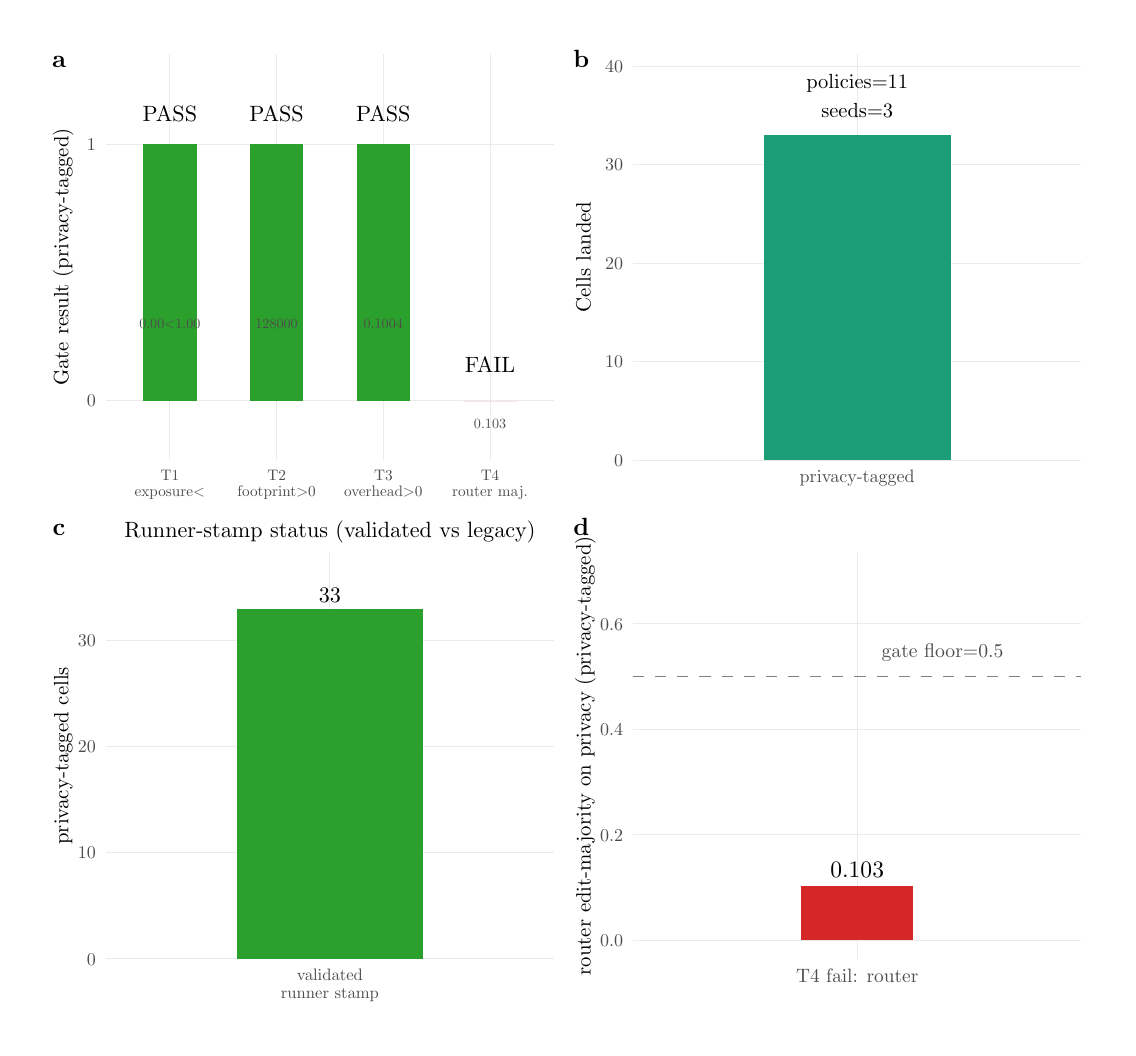
\begin{tikzpicture}[x=1pt,y=1pt]
\definecolor{fillColor}{RGB}{255,255,255}
\path[use as bounding box,fill=fillColor,fill opacity=0.00] (0,0) rectangle (390.26,361.35);
\begin{scope}
\path[clip] (  0.00,  0.00) rectangle (390.26,361.35);
\definecolor{drawColor}{RGB}{255,255,255}
\definecolor{fillColor}{RGB}{255,255,255}

\path[draw=drawColor,line width= 0.6pt,line join=round,line cap=round,fill=fillColor] (  0.00,  0.00) rectangle (390.26,361.35);
\end{scope}
\begin{scope}
\path[clip] (  5.50,186.70) rectangle (194.23,355.85);
\definecolor{fillColor}{RGB}{255,255,255}

\path[fill=fillColor] (  5.50,186.70) rectangle (194.23,355.85);
\end{scope}
\begin{scope}
\path[clip] (194.23,186.70) rectangle (384.76,355.85);
\definecolor{fillColor}{RGB}{255,255,255}

\path[fill=fillColor] (194.23,186.70) rectangle (384.76,355.85);
\end{scope}
\begin{scope}
\path[clip] (  5.50,  5.50) rectangle (194.23,186.70);
\definecolor{fillColor}{RGB}{255,255,255}

\path[fill=fillColor] (  5.50,  5.50) rectangle (194.23,186.70);
\end{scope}
\begin{scope}
\path[clip] (194.23,  5.50) rectangle (384.76,186.70);
\definecolor{fillColor}{RGB}{255,255,255}

\path[fill=fillColor] (194.23,  5.50) rectangle (384.76,186.70);
\end{scope}
\begin{scope}
\path[clip] ( 28.22,205.10) rectangle (190.23,351.85);
\definecolor{drawColor}{gray}{0.92}

\path[draw=drawColor,line width= 0.4pt,line join=round] ( 28.22,226.59) --
	(190.23,226.59);

\path[draw=drawColor,line width= 0.4pt,line join=round] ( 28.22,319.24) --
	(190.23,319.24);

\path[draw=drawColor,line width= 0.4pt,line join=round] ( 51.37,205.10) --
	( 51.37,351.85);

\path[draw=drawColor,line width= 0.4pt,line join=round] ( 89.94,205.10) --
	( 89.94,351.85);

\path[draw=drawColor,line width= 0.4pt,line join=round] (128.51,205.10) --
	(128.51,351.85);

\path[draw=drawColor,line width= 0.4pt,line join=round] (167.08,205.10) --
	(167.08,351.85);
\definecolor{fillColor}{RGB}{44,160,44}

\path[fill=fillColor] ( 41.72,226.59) rectangle ( 61.01,319.24);

\path[fill=fillColor] ( 80.29,226.59) rectangle ( 99.58,319.24);

\path[fill=fillColor] (118.87,226.59) rectangle (138.15,319.24);
\definecolor{fillColor}{RGB}{214,39,40}

\path[fill=fillColor] (157.44,226.59) rectangle (176.73,226.59);
\definecolor{drawColor}{RGB}{0,0,0}

\node[text=drawColor,anchor=base,inner sep=0pt, outer sep=0pt, scale=  0.80] at ( 51.37,327.61) {PASS};

\node[text=drawColor,anchor=base,inner sep=0pt, outer sep=0pt, scale=  0.80] at ( 89.94,327.61) {PASS};

\node[text=drawColor,anchor=base,inner sep=0pt, outer sep=0pt, scale=  0.80] at (128.51,327.61) {PASS};

\node[text=drawColor,anchor=base,inner sep=0pt, outer sep=0pt, scale=  0.80] at (167.08,236.82) {FAIL};
\definecolor{drawColor}{gray}{0.30}

\node[text=drawColor,anchor=base,inner sep=0pt, outer sep=0pt, scale=  0.51] at ( 51.37,252.62) {0.00$<$1.00};

\node[text=drawColor,anchor=base,inner sep=0pt, outer sep=0pt, scale=  0.51] at ( 89.94,252.62) {128000};

\node[text=drawColor,anchor=base,inner sep=0pt, outer sep=0pt, scale=  0.51] at (128.51,252.62) {0.1004};

\node[text=drawColor,anchor=base,inner sep=0pt, outer sep=0pt, scale=  0.51] at (167.08,216.49) {0.103};
\end{scope}
\begin{scope}
\path[clip] (  0.00,  0.00) rectangle (390.26,361.35);
\definecolor{drawColor}{gray}{0.30}

\node[text=drawColor,anchor=base east,inner sep=0pt, outer sep=0pt, scale=  0.65] at ( 24.62,224.35) {0};

\node[text=drawColor,anchor=base east,inner sep=0pt, outer sep=0pt, scale=  0.65] at ( 24.62,317.00) {1};
\end{scope}
\begin{scope}
\path[clip] (  0.00,  0.00) rectangle (390.26,361.35);
\definecolor{drawColor}{gray}{0.30}

\node[text=drawColor,anchor=base,inner sep=0pt, outer sep=0pt, scale=  0.55] at ( 51.37,197.71) {T1};

\node[text=drawColor,anchor=base,inner sep=0pt, outer sep=0pt, scale=  0.55] at ( 51.37,191.77) {exposure$<$};

\node[text=drawColor,anchor=base,inner sep=0pt, outer sep=0pt, scale=  0.55] at ( 89.94,197.71) {T2};

\node[text=drawColor,anchor=base,inner sep=0pt, outer sep=0pt, scale=  0.55] at ( 89.94,191.77) {footprint$>$0};

\node[text=drawColor,anchor=base,inner sep=0pt, outer sep=0pt, scale=  0.55] at (128.51,197.71) {T3};

\node[text=drawColor,anchor=base,inner sep=0pt, outer sep=0pt, scale=  0.55] at (128.51,191.77) {overhead$>$0};

\node[text=drawColor,anchor=base,inner sep=0pt, outer sep=0pt, scale=  0.55] at (167.08,197.71) {T4};

\node[text=drawColor,anchor=base,inner sep=0pt, outer sep=0pt, scale=  0.55] at (167.08,191.77) {router maj.};
\end{scope}
\begin{scope}
\path[clip] (  0.00,  0.00) rectangle (390.26,361.35);
\definecolor{drawColor}{RGB}{0,0,0}

\node[text=drawColor,rotate= 90.00,anchor=base,inner sep=0pt, outer sep=0pt, scale=  0.75] at ( 14.67,278.47) {Gate result (privacy-tagged)};
\end{scope}
\begin{scope}
\path[clip] (  0.00,  0.00) rectangle (390.26,361.35);
\definecolor{drawColor}{RGB}{0,0,0}

\node[text=drawColor,anchor=base,inner sep=0pt, outer sep=0pt, scale=  0.90] at ( 11.31,347.13) {\bfseries a};
\end{scope}
\begin{scope}
\path[clip] (218.75,205.10) rectangle (380.76,351.85);
\definecolor{drawColor}{gray}{0.92}

\path[draw=drawColor,line width= 0.4pt,line join=round] (218.75,205.10) --
	(380.76,205.10);

\path[draw=drawColor,line width= 0.4pt,line join=round] (218.75,240.67) --
	(380.76,240.67);

\path[draw=drawColor,line width= 0.4pt,line join=round] (218.75,276.25) --
	(380.76,276.25);

\path[draw=drawColor,line width= 0.4pt,line join=round] (218.75,311.83) --
	(380.76,311.83);

\path[draw=drawColor,line width= 0.4pt,line join=round] (218.75,347.40) --
	(380.76,347.40);

\path[draw=drawColor,line width= 0.4pt,line join=round] (299.76,205.10) --
	(299.76,351.85);
\definecolor{fillColor}{RGB}{27,158,119}

\path[fill=fillColor] (266.00,205.10) rectangle (333.51,322.50);
\definecolor{drawColor}{RGB}{0,0,0}

\node[text=drawColor,anchor=base,inner sep=0pt, outer sep=0pt, scale=  0.74] at (299.76,339.45) {policies=11};

\node[text=drawColor,anchor=base,inner sep=0pt, outer sep=0pt, scale=  0.74] at (299.76,328.80) {seeds=3};
\end{scope}
\begin{scope}
\path[clip] (  0.00,  0.00) rectangle (390.26,361.35);
\definecolor{drawColor}{gray}{0.30}

\node[text=drawColor,anchor=base east,inner sep=0pt, outer sep=0pt, scale=  0.65] at (215.15,202.86) {0};

\node[text=drawColor,anchor=base east,inner sep=0pt, outer sep=0pt, scale=  0.65] at (215.15,238.43) {10};

\node[text=drawColor,anchor=base east,inner sep=0pt, outer sep=0pt, scale=  0.65] at (215.15,274.01) {20};

\node[text=drawColor,anchor=base east,inner sep=0pt, outer sep=0pt, scale=  0.65] at (215.15,309.59) {30};

\node[text=drawColor,anchor=base east,inner sep=0pt, outer sep=0pt, scale=  0.65] at (215.15,345.16) {40};
\end{scope}
\begin{scope}
\path[clip] (  0.00,  0.00) rectangle (390.26,361.35);
\definecolor{drawColor}{gray}{0.30}

\node[text=drawColor,anchor=base,inner sep=0pt, outer sep=0pt, scale=  0.65] at (299.76,197.02) {privacy-tagged};
\end{scope}
\begin{scope}
\path[clip] (  0.00,  0.00) rectangle (390.26,361.35);
\definecolor{drawColor}{RGB}{0,0,0}

\node[text=drawColor,rotate= 90.00,anchor=base,inner sep=0pt, outer sep=0pt, scale=  0.75] at (203.39,278.47) {Cells landed};
\end{scope}
\begin{scope}
\path[clip] (  0.00,  0.00) rectangle (390.26,361.35);
\definecolor{drawColor}{RGB}{0,0,0}

\node[text=drawColor,anchor=base,inner sep=0pt, outer sep=0pt, scale=  0.90] at (200.05,347.13) {\bfseries b};
\end{scope}
\begin{scope}
\path[clip] ( 28.22, 24.88) rectangle (190.23,171.63);
\definecolor{drawColor}{gray}{0.92}

\path[draw=drawColor,line width= 0.4pt,line join=round] ( 28.22, 24.88) --
	(190.23, 24.88);

\path[draw=drawColor,line width= 0.4pt,line join=round] ( 28.22, 63.22) --
	(190.23, 63.22);

\path[draw=drawColor,line width= 0.4pt,line join=round] ( 28.22,101.55) --
	(190.23,101.55);

\path[draw=drawColor,line width= 0.4pt,line join=round] ( 28.22,139.89) --
	(190.23,139.89);

\path[draw=drawColor,line width= 0.4pt,line join=round] (109.22, 24.88) --
	(109.22,171.63);
\definecolor{fillColor}{RGB}{44,160,44}

\path[fill=fillColor] ( 75.47, 24.88) rectangle (142.98,151.39);
\definecolor{drawColor}{RGB}{0,0,0}

\node[text=drawColor,anchor=base,inner sep=0pt, outer sep=0pt, scale=  0.80] at (109.22,153.59) {33};
\end{scope}
\begin{scope}
\path[clip] (  0.00,  0.00) rectangle (390.26,361.35);
\definecolor{drawColor}{gray}{0.30}

\node[text=drawColor,anchor=base east,inner sep=0pt, outer sep=0pt, scale=  0.65] at ( 24.62, 22.64) {0};

\node[text=drawColor,anchor=base east,inner sep=0pt, outer sep=0pt, scale=  0.65] at ( 24.62, 60.98) {10};

\node[text=drawColor,anchor=base east,inner sep=0pt, outer sep=0pt, scale=  0.65] at ( 24.62, 99.31) {20};

\node[text=drawColor,anchor=base east,inner sep=0pt, outer sep=0pt, scale=  0.65] at ( 24.62,137.65) {30};
\end{scope}
\begin{scope}
\path[clip] (  0.00,  0.00) rectangle (390.26,361.35);
\definecolor{drawColor}{gray}{0.30}

\node[text=drawColor,anchor=base,inner sep=0pt, outer sep=0pt, scale=  0.60] at (109.22, 17.15) {validated};

\node[text=drawColor,anchor=base,inner sep=0pt, outer sep=0pt, scale=  0.60] at (109.22, 10.67) {runner stamp};
\end{scope}
\begin{scope}
\path[clip] (  0.00,  0.00) rectangle (390.26,361.35);
\definecolor{drawColor}{RGB}{0,0,0}

\node[text=drawColor,rotate= 90.00,anchor=base,inner sep=0pt, outer sep=0pt, scale=  0.75] at ( 14.67, 98.26) {privacy-tagged cells};
\end{scope}
\begin{scope}
\path[clip] (  0.00,  0.00) rectangle (390.26,361.35);
\definecolor{drawColor}{RGB}{0,0,0}

\node[text=drawColor,anchor=base,inner sep=0pt, outer sep=0pt, scale=  0.80] at (109.22,177.19) {Runner-stamp status (validated vs legacy)};
\end{scope}
\begin{scope}
\path[clip] (  0.00,  0.00) rectangle (390.26,361.35);
\definecolor{drawColor}{RGB}{0,0,0}

\node[text=drawColor,anchor=base,inner sep=0pt, outer sep=0pt, scale=  0.90] at ( 11.31,177.86) {\bfseries c};
\end{scope}
\begin{scope}
\path[clip] (218.75, 24.88) rectangle (380.76,171.63);
\definecolor{drawColor}{gray}{0.92}

\path[draw=drawColor,line width= 0.4pt,line join=round] (218.75, 31.55) --
	(380.76, 31.55);

\path[draw=drawColor,line width= 0.4pt,line join=round] (218.75, 69.67) --
	(380.76, 69.67);

\path[draw=drawColor,line width= 0.4pt,line join=round] (218.75,107.79) --
	(380.76,107.79);

\path[draw=drawColor,line width= 0.4pt,line join=round] (218.75,145.90) --
	(380.76,145.90);

\path[draw=drawColor,line width= 0.4pt,line join=round] (299.76, 24.88) --
	(299.76,171.63);
\definecolor{fillColor}{RGB}{214,39,40}

\path[fill=fillColor] (279.51, 31.55) rectangle (320.01, 51.19);
\definecolor{drawColor}{gray}{0.50}

\path[draw=drawColor,line width= 0.5pt,dash pattern=on 4pt off 4pt ,line join=round] (218.75,126.84) -- (380.76,126.84);
\definecolor{drawColor}{gray}{0.30}

\node[text=drawColor,anchor=base west,inner sep=0pt, outer sep=0pt, scale=  0.71] at (308.57,133.92) {gate floor=0.5};
\definecolor{drawColor}{RGB}{0,0,0}

\node[text=drawColor,anchor=base,inner sep=0pt, outer sep=0pt, scale=  0.85] at (299.76, 54.13) {0.103};
\end{scope}
\begin{scope}
\path[clip] (  0.00,  0.00) rectangle (390.26,361.35);
\definecolor{drawColor}{gray}{0.30}

\node[text=drawColor,anchor=base east,inner sep=0pt, outer sep=0pt, scale=  0.65] at (215.15, 29.31) {0.0};

\node[text=drawColor,anchor=base east,inner sep=0pt, outer sep=0pt, scale=  0.65] at (215.15, 67.43) {0.2};

\node[text=drawColor,anchor=base east,inner sep=0pt, outer sep=0pt, scale=  0.65] at (215.15,105.55) {0.4};

\node[text=drawColor,anchor=base east,inner sep=0pt, outer sep=0pt, scale=  0.65] at (215.15,143.67) {0.6};
\end{scope}
\begin{scope}
\path[clip] (  0.00,  0.00) rectangle (390.26,361.35);
\definecolor{drawColor}{gray}{0.30}

\node[text=drawColor,anchor=base,inner sep=0pt, outer sep=0pt, scale=  0.70] at (299.76, 16.46) {T4 fail: router};
\end{scope}
\begin{scope}
\path[clip] (  0.00,  0.00) rectangle (390.26,361.35);
\definecolor{drawColor}{RGB}{0,0,0}

\node[text=drawColor,rotate= 90.00,anchor=base,inner sep=0pt, outer sep=0pt, scale=  0.75] at (203.39, 98.26) {router edit-majority on privacy (privacy-tagged)};
\end{scope}
\begin{scope}
\path[clip] (  0.00,  0.00) rectangle (390.26,361.35);
\definecolor{drawColor}{RGB}{0,0,0}

\node[text=drawColor,anchor=base,inner sep=0pt, outer sep=0pt, scale=  0.90] at (200.05,177.86) {\bfseries d};
\end{scope}
\end{tikzpicture}
